% ============================================================
% BSP Final Report - ACM-style two-column layout
% University of Luxembourg, 2025/26
% ============================================================
\documentclass[10pt, twocolumn, a4paper]{article}

% --- Core packages (all standard, no exotic dependencies) ---
\usepackage[T1]{fontenc}
\usepackage[utf8]{inputenc}
\usepackage[margin=1.9cm, top=2.2cm, bottom=2.4cm, columnsep=0.6cm]{geometry}
\usepackage{mathptmx}
\usepackage{booktabs}
\usepackage{graphicx}
\usepackage{xcolor}
\usepackage[hidelinks]{hyperref}
\usepackage{enumitem}
\usepackage{titlesec}
\usepackage{fancyhdr}
\usepackage{caption}

% --- Section formatting ---
\titleformat{\section}{\normalfont\large\bfseries}{\thesection.}{0.5em}{}
\titleformat{\subsection}{\normalfont\normalsize\bfseries}{\thesubsection.}{0.5em}{}
\titlespacing*{\section}{0pt}{8pt plus 2pt}{4pt plus 1pt}
\titlespacing*{\subsection}{0pt}{6pt plus 2pt}{2pt plus 1pt}

% --- Caption formatting ---
\captionsetup{font=small, labelfont=bf, skip=4pt}

% --- List spacing ---
\setlist[itemize]{noitemsep, topsep=3pt, leftmargin=*}

% --- Header/Footer ---
\pagestyle{fancy}
\fancyhf{}
\fancyhead[C]{\small\textit{BSP S2 (Academic Year 2025/26), University of Luxembourg}}
\fancyfoot[C]{\thepage}
\renewcommand{\headrulewidth}{0.4pt}

\setlength{\parskip}{0pt}
\setlength{\parindent}{9pt}

%% ============================================================
\begin{document}
%% ============================================================

% --- Title block ---
\twocolumn[{%
\begin{center}
  {\LARGE\bfseries Large Language Models for Clinical Diagnosis\\[3pt]
  and Treatment Recommendation}\\[8pt]
  {\normalsize Bachelor Semester Project S2 (Academic Year 2025/26), University of Luxembourg}\\[10pt]
  \begin{tabular}{ccc}
    \textbf{Can Yildiz} & \textbf{Nina Vojtassak} & \textbf{Tuna Karakus} \\
    \small can.yildiz.001@student.uni.lu &
    \small nina.vojtassak.001@student.uni.lu &
    \small tuna.karakus.001@student.uni.lu \\
  \end{tabular}\\[12pt]
  \begin{minipage}{0.92\linewidth}
  \begin{center}\textbf{Abstract}\end{center}
  \small
Clinical decision support systems powered by large language models represent a promising frontier in medical artificial intelligence. This paper presents Project Omega, a systematic comparative evaluation of Meta's LLaMA-3.3-70B and Google's Gemma-4-31B on the task of clinical diagnosis hypothesization and treatment recommendation. Using a cohort of 2,000 patient admissions from the MIMIC-IV clinical database, we construct structured prompts from electronic health records and evaluate model outputs across output verbosity, drug overlap, BLEU and ROUGE-1/2/L scores, and four clinical quality dimensions (accuracy, completeness, safety, usefulness) assessed by an autonomous LLM evaluator (GPT-OSS 120B). We additionally conduct a temperature sensitivity experiment on 1,000 patients and apply LIME-based explainability analysis. Gemma-4-31B wins 97.9\% of head-to-head evaluations while simultaneously scoring lower on BLEU and ROUGE, revealing a fundamental limitation of n-gram metrics for clinical text generation tasks.
  \end{minipage}\\[14pt]
  \rule{0.92\linewidth}{0.4pt}\\[8pt]
\end{center}
}]

%% =====================================================================
\section{Introduction}
%% =====================================================================

The integration of artificial intelligence into clinical workflows has long been a central ambition of biomedical informatics. Electronic health records contain rich, longitudinal data spanning diagnoses, laboratory measurements, vital signs, pharmacological histories, and procedural notes. Transforming this data into actionable clinical recommendations is a task that historically required years of specialist training, yet represents a natural target for modern language models trained on vast biomedical corpora~\cite{llmclinical}.

Large language models have demonstrated remarkable capabilities on structured medical benchmarks. GPT-4 achieves passing scores on the United States Medical Licensing Examination~\cite{gpt4med}, and biomedical variants such as BioBERT~\cite{biobert} and ClinicalBERT~\cite{clinicalbert} have established strong baselines on clinical information extraction tasks. However, standardized multiple-choice examinations do not capture the open-ended complexity of real clinical reasoning: generating a differential diagnosis list, proposing a treatment plan, identifying drug interactions, and communicating safety concerns to a clinical practitioner.

The rapid proliferation of open-weight language models has made it feasible to deploy powerful inference pipelines without proprietary APIs. Meta's LLaMA family~\cite{llama3} and Google's Gemma models~\cite{gemma} now offer strong instruction-following capabilities at scales accessible to academic research groups. Yet systematic comparative studies of these models on realistic clinical tasks grounded in real patient data remain scarce.

This paper addresses this gap through Project Omega, a pipeline-based evaluation framework built on the MIMIC-IV clinical database~\cite{mimic4}. Our contributions are:

\begin{itemize}
  \item \textbf{Pipeline Design.} A scalable Python pipeline processes structured EHR data from a DuckDB-indexed MIMIC-IV database, constructs multi-section clinical prompts, and queries two LLMs across 2,000 patient admissions.
  \item \textbf{Multi-Dimensional Evaluation.} Outputs are evaluated across output verbosity, drug overlap ratios, BLEU and ROUGE-1/2/L scores, and four clinical quality axes assessed by an autonomous GPT-OSS 120B evaluator~\cite{llmjudge}.
  \item \textbf{Temperature Sensitivity.} The effect of the generation temperature on Gemma-4-31B output quality is investigated across 1,000 patients at three settings.
  \item \textbf{Explainability.} LIME~\cite{lime} is applied to identify which prompt sections most influence each model's output behavior.
\end{itemize}

Our central finding is a counterintuitive reversal of rankings between lexical similarity metrics and clinical quality assessments. LLaMA-3.3-70B achieves higher BLEU and ROUGE scores due to its concise outputs, yet Gemma-4-31B wins 97.9\% of head-to-head clinical evaluations. This result has direct methodological implications for the evaluation of clinical text generation systems.

%% =====================================================================
\section{Related Work}
%% =====================================================================

\subsection{NLP in Clinical Medicine}
Natural language processing has been applied to clinical text for decades, beginning with rule-based systems for named entity recognition in discharge summaries. The introduction of transformer architectures fundamentally transformed the field. BioBERT~\cite{biobert} and ClinicalBERT~\cite{clinicalbert} demonstrated that domain-adaptive pretraining on biomedical and clinical corpora yields substantial gains on downstream clinical tasks including NER, relation extraction, and question answering.

\subsection{LLMs on Medical Tasks}
Singhal et al.~\cite{llmclinical} show that instruction-tuned language models encode substantial clinical knowledge and achieve competitive performance on medical question-answering. Nori et al.~\cite{gpt4med} demonstrate GPT-4's ability to pass standardized medical licensing examinations, while Jin et al.~\cite{medqa} present large-scale question-answering datasets demonstrating the gap between model capabilities and expert human performance. Performance on free-form clinical generation situated within real patient records, however, remains considerably less studied. Our work directly targets this gap by constructing prompts from structured EHR data rather than from curated examination questions.

\subsection{LLM-as-Judge Evaluation}
The LLM-as-Judge paradigm, formalized by Zheng et al.~\cite{llmjudge} through the MT-Bench framework, proposes using a capable language model as an autonomous preference evaluator. The authors demonstrate strong agreement between GPT-4 judgments and human annotations across open-ended tasks. We adopt this paradigm using GPT-OSS 120B as our evaluator, scoring model outputs on four clinical quality dimensions across all 2,000 patients.

\subsection{Evaluation Metrics for Text Generation}
BLEU~\cite{bleu} and ROUGE~\cite{rouge} remain the dominant automatic metrics for text generation evaluation. Both measure lexical n-gram overlap between generated text and a reference string. Their applicability to clinical text is contested: a comprehensive clinical recommendation including treatment rationales, safety warnings, and procedural guidance will naturally show lower BLEU and ROUGE scores relative to a terse output, even if it is clinically superior. Our results empirically confirm this limitation.

%% =====================================================================
\section{Methodology}
%% =====================================================================

\subsection{Dataset and Patient Cohort}
We use the MIMIC-IV clinical database~\cite{mimic4}, a freely accessible collection of de-identified health records from over 40,000 patients admitted to the critical care units of Beth Israel Deaconess Medical Center between 2008 and 2024, locally indexed using DuckDB.

Patient eligibility requires at least one ICD diagnosis code, at least one laboratory event, and at least one prescription record. From the eligible pool, a reproducible random cohort of 2,000 patients is drawn using a seeded shuffle (seed = 42). Cohort identifiers are persisted to CSV to guarantee identical patient selection across pipeline restarts.

\subsection{Two-Phase Data Loading}
To maintain a constant memory footprint, we adopt a two-phase architecture. Phase 1 retrieves patient identifiers, demographics, and all ICD-coded diagnoses in a lightweight query held in memory throughout the run. Phase 2 loads, for each batch of 50 patients, laboratory results with human-readable labels, prescriptions, ICU stay records, chartevents vitals (heart rate, SpO$_2$, temperature, blood pressure, respiratory rate), OMR anthropometrics, ICD-coded procedures, and microbiology culture results. Batch data is released after each iteration.

\subsection{Prompt Construction}
Clinical data for each patient is assembled into a structured, eight-section prompt: Patient Demographics, Diagnoses (primary flagged separately), Laboratory Results (up to 15 most recent numeric measurements), ICU Vitals (up to 12 chartevents measurements), Vital Signs and Anthropometrics (OMR records), Procedures Performed, Microbiology and Culture Results, and ICU Stay duration.

The task instruction requires each model to respond in exactly four structured sections: (1) Additional Diagnosis Hypotheses, listing 3 to 5 differential or comorbid diagnoses with clinical rationales; (2) Recommended Treatments with drug names and typical doses; (3) Safety Flags and Drug Interactions; and (4) Confidence Level with a one-sentence explanation.

\subsection{Models}
\textbf{LLaMA-3.3-70B-Versatile} is Meta's 70-billion-parameter decoder-only transformer~\cite{llama3}, accessed via the Groq inference API. \textbf{Gemma-4-31B-IT} is Google's 31-billion-parameter instruction-tuned model~\cite{gemma}, accessed via the Google Generative AI API. Both models use temperature $T = 0.3$ and a maximum of 2,500 output tokens. The autonomous evaluator \textbf{GPT-OSS 120B} is queried at temperature $T = 0.1$ with up to 3,000 tokens.

\subsection{Drug Overlap Analysis}
True prescribed medications are retrieved from the MIMIC-IV prescriptions table. A fuzzy string matching algorithm (Python difflib SequenceMatcher, threshold $\geq 0.75$) compares drug tokens extracted from model outputs against the ground-truth prescription list, yielding absolute match counts and recall ratios normalized by the number of true prescriptions.

\subsection{Temperature Sensitivity Experiment}
Gemma-4-31B is re-queried on a subset of 1,000 patients at three temperature settings $T \in \{0.1, 0.5, 1.0\}$. BLEU and ROUGE-1 scores are computed against the patient's concatenated ICD diagnosis descriptions, producing 3,000 evaluation pairs.

%% =====================================================================
\section{Evaluation Strategy}
%% =====================================================================

\subsection{Lexical Similarity}
BLEU~\cite{bleu} is computed using NLTK's \texttt{sentence\_bleu} with Chen and Cherry smoothing (Method 1). ROUGE-1, ROUGE-2, and ROUGE-L~\cite{rouge} are computed using the \texttt{rouge-score} library. Reference text is the concatenated ICD long-title diagnosis string for each admission.

\subsection{LLM-as-Judge}
GPT-OSS 120B scores each pair of model outputs on four axes, each from 1 to 25 (total out of 100):

\begin{itemize}
  \item \textbf{Clinical Accuracy.} Correctness of differential diagnoses, recommended drugs, and dosing.
  \item \textbf{Completeness.} Coverage of all clinically relevant aspects without omitting critical information.
  \item \textbf{Safety.} Identification of drug interactions, contraindications, and safety warnings.
  \item \textbf{Practical Usefulness.} Clarity, structure, and actionability for a clinical practitioner.
\end{itemize}

The evaluator additionally designates a head-to-head winner (model1, model2, or tie) and provides a short comparison rationale returned as structured JSON parsed programmatically.

%% =====================================================================
\section{Results and Analysis}
%% =====================================================================

Figure~\ref{fig:dashboard} presents the full evaluation dashboard. Table~\ref{tab:results} summarizes quantitative results.

\begin{table}[h]
\centering
\caption{Comparative results ($n = 2{,}000$). BLEU and ROUGE values are medians. Evaluator scores are medians as percentages of maximum.}
\label{tab:results}
\small
\renewcommand{\arraystretch}{1.1}
\begin{tabular}{lcc}
\toprule
\textbf{Metric} & \textbf{LLaMA-70B} & \textbf{Gemma-31B} \\
\midrule
Output length (chars) & 2,100 & 4,500 \\
Drug overlap (count) & 1.9 & 2.1 \\
Drug overlap (\% true Rx) & 3.8\% & 4.2\% \\
\midrule
BLEU & 0.052 & 0.018 \\
ROUGE-1 & 0.220 & 0.121 \\
ROUGE-2 & 0.071 & 0.040 \\
ROUGE-L & 0.135 & 0.105 \\
\midrule
Evaluator total (\%) & 50 & 75 \\
Accuracy (\%) & 65 & 85 \\
Safety (\%) & 56 & 85 \\
Completeness (\%) & 48 & 80 \\
Usefulness (\%) & 48 & 82 \\
\midrule
Head-to-head wins & 38 (1.9\%) & 1,959 (97.9\%) \\
\bottomrule
\end{tabular}
\end{table}

\begin{figure*}[t]
  \centering
  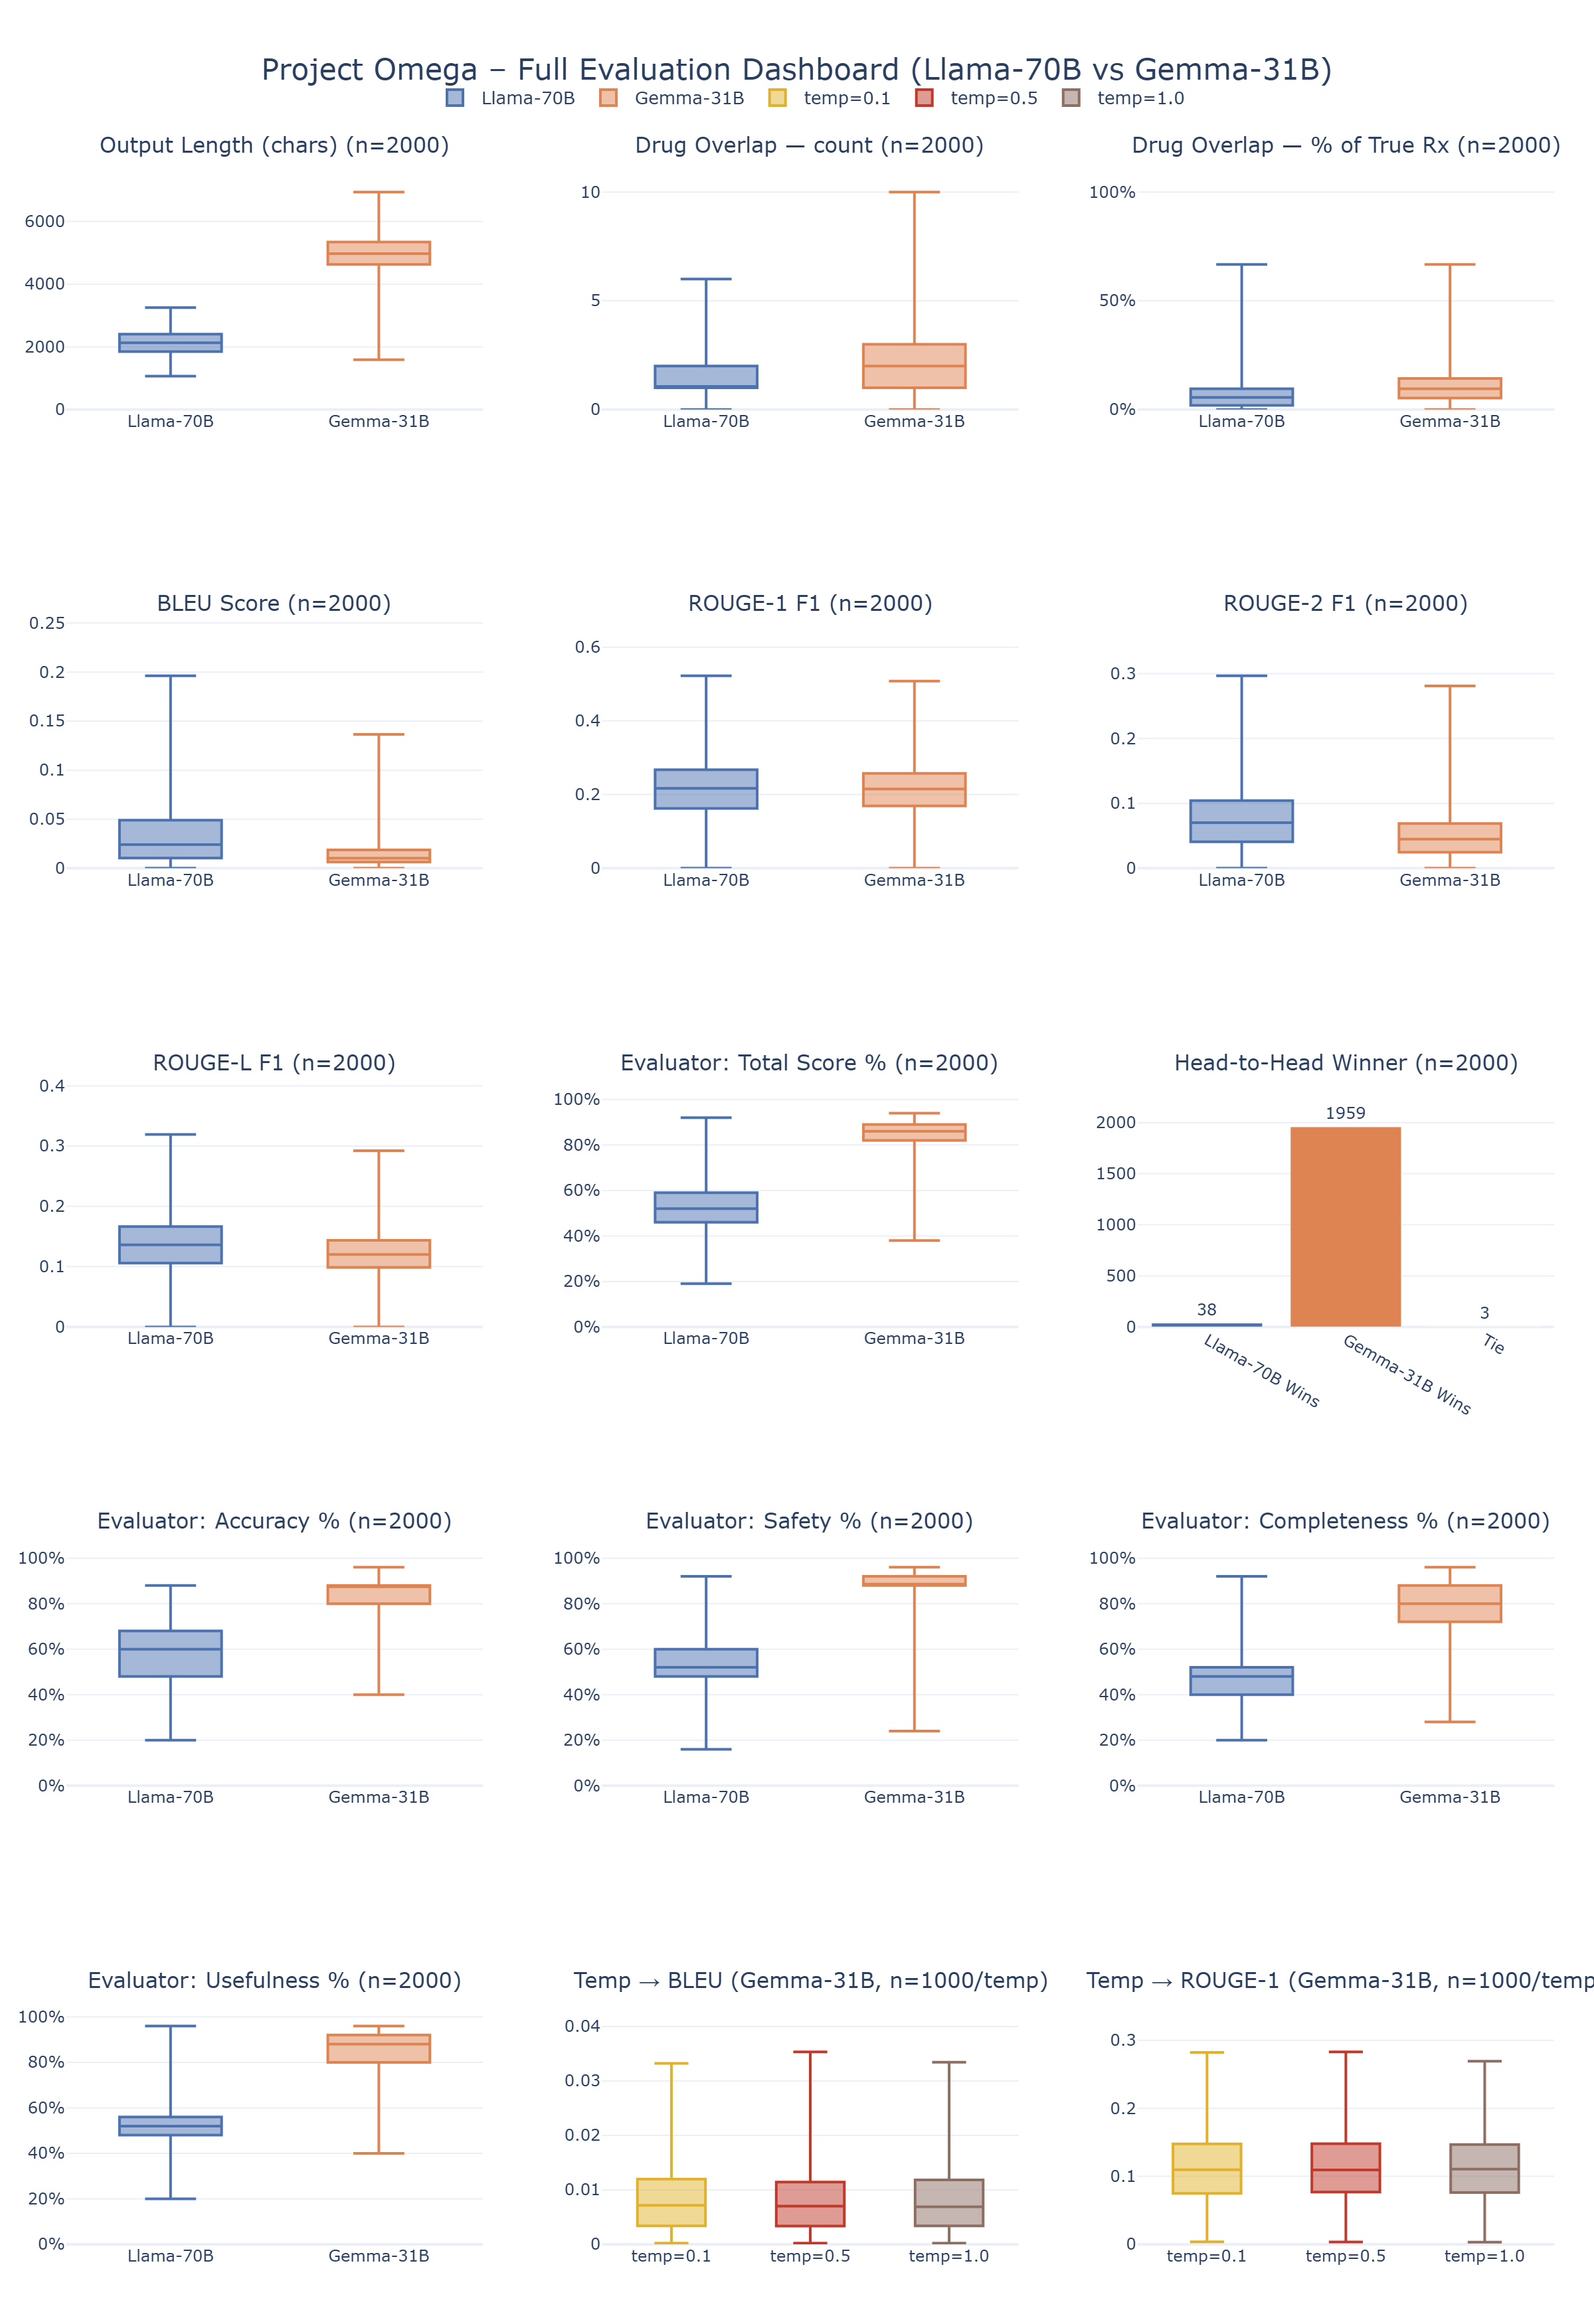
\includegraphics[width=\textwidth]{figures/evaluation_dashboard.png}
  \caption{Full evaluation dashboard for 2,000 MIMIC-IV patients. Rows 1 and 2: output statistics and lexical similarity metrics. Row 3: head-to-head winner counts and evaluator total scores. Rows 4 and 5: evaluator subscores and temperature sensitivity analysis (Gemma-4-31B, $n = 1{,}000$ per temperature).}
  \label{fig:dashboard}
\end{figure*}

\subsection{Output Verbosity}
A pronounced difference in output verbosity characterizes the two models. LLaMA-3.3-70B produces consistently concise outputs (median $\approx 2{,}100$ characters, IQR 1,800-2,300), while Gemma-4-31B generates substantially longer responses (median $\approx 4{,}500$ characters, IQR 3,500-5,000). This $2.1\times$ difference in output length is the primary driver of the divergence in n-gram similarity scores discussed below.

\subsection{Drug Overlap}
Both models achieve modest drug overlap counts (median 2 matched drugs per patient), reflecting the inherent difficulty of exact pharmacological recommendation from ICD diagnosis codes alone. Drug overlap percentage remains below 10\% for both models, consistent with findings in related LLM pharmacology studies. Gemma's wider output distribution yields a marginally higher count at the upper quartile, suggesting its more comprehensive outputs occasionally recover additional relevant medications.

\subsection{Lexical Similarity and the Brevity Effect}
LLaMA-3.3-70B achieves higher median BLEU (0.052 vs. 0.018) and ROUGE-1 (0.220 vs. 0.121) scores than Gemma-4-31B. The explanation lies in the \textit{brevity effect}: LLaMA's shorter, diagnosis-focused outputs contain a higher proportion of ICD-related vocabulary, yielding greater lexical overlap with the ICD reference strings. Gemma's comprehensive outputs, which include treatment plans, drug interaction warnings, and procedural guidance, contain proportionally less diagnosis-specific vocabulary and are penalized by n-gram precision metrics.

This result has a direct methodological implication: BLEU and ROUGE should not serve as primary quality indicators for open-ended clinical generation tasks where reference strings are concise ICD descriptions.

\subsection{Clinical Quality Evaluation}
The GPT-OSS 120B evaluator reveals a decisive advantage for Gemma-4-31B across all four quality dimensions. Gemma achieves a median total score of approximately 75\% versus LLaMA's 50\%. In head-to-head comparisons, Gemma wins 1,959 of 2,000 evaluations (97.9\%), LLaMA wins 38 (1.9\%), and 3 result in a tie.

The largest performance gaps appear in Completeness (Gemma 80\% vs. LLaMA 48\%) and Usefulness (Gemma 82\% vs. LLaMA 48\%), confirming that Gemma's verbosity translates into genuine clinical value. Safety scores differ substantially (Gemma 85\% vs. LLaMA 56\%), suggesting LLaMA more frequently omits drug interaction warnings and contraindication notices.

\subsection{Temperature Sensitivity}

Table~\ref{tab:temperature} shows temperature's effect on Gemma output quality. BLEU scores remain uniformly low ($\approx 0.010$-$0.011$) across all three temperatures. ROUGE-1 shows a slight upward trend from $T = 0.1$ (median $\approx 0.100$) to $T \in \{0.5, 1.0\}$ (median $\approx 0.122$), suggesting that higher temperatures introduce vocabulary diversity that marginally increases recall. Overall, Gemma-4-31B is largely robust to this hyperparameter within the tested range.

\begin{table}[h]
\centering
\caption{Temperature sensitivity for Gemma-4-31B ($n = 1{,}000$ per setting). Values are medians.}
\label{tab:temperature}
\small
\begin{tabular}{lcc}
\toprule
\textbf{Temperature} & \textbf{BLEU} & \textbf{ROUGE-1} \\
\midrule
0.1 & 0.010 & 0.100 \\
0.5 & 0.011 & 0.122 \\
1.0 & 0.011 & 0.123 \\
\bottomrule
\end{tabular}
\end{table}

%% =====================================================================
\section{Explainability Analysis}
%% =====================================================================

\subsection{LIME Setup}
To understand which sections of the clinical prompt most influence each model's response, we apply LIME~\cite{lime} to 50 randomly sampled patients per model. For each patient, 800 perturbed prompt variants are generated by randomly masking token subsets. Each perturbed prompt is submitted to the model and the resulting output is compared to the original output using TF-IDF cosine similarity. A linear surrogate model fitted to these input-output pairs identifies the most influential tokens.

An important methodological note: this setup measures \textit{lexical influence}, specifically whether a token's presence causes the model to produce vocabulary similar to its unperturbed output. This constitutes a lexical-overlap proxy for explainability rather than a measure of semantic influence or causal reasoning.

\subsection{Results}
Figure~\ref{fig:lime} displays the top globally influential words aggregated across all sampled patients for each model. For both LLaMA-3.3-70B and Gemma-4-31B, tokens from the Diagnoses and Laboratory Results sections consistently rank among the most influential. This confirms that both models anchor primarily on clinical diagnostic context rather than on demographic information or procedural history.

Section-level heatmap analysis reveals a notable difference: LLaMA's outputs are most strongly influenced by primary diagnosis terminology, reflecting its concise, diagnosis-centric generation style. Gemma exhibits more distributed influence across the Diagnoses, Laboratory Results, and Vital Signs sections, consistent with its broader, more integrative output behavior.

\begin{figure*}[t]
  \centering
  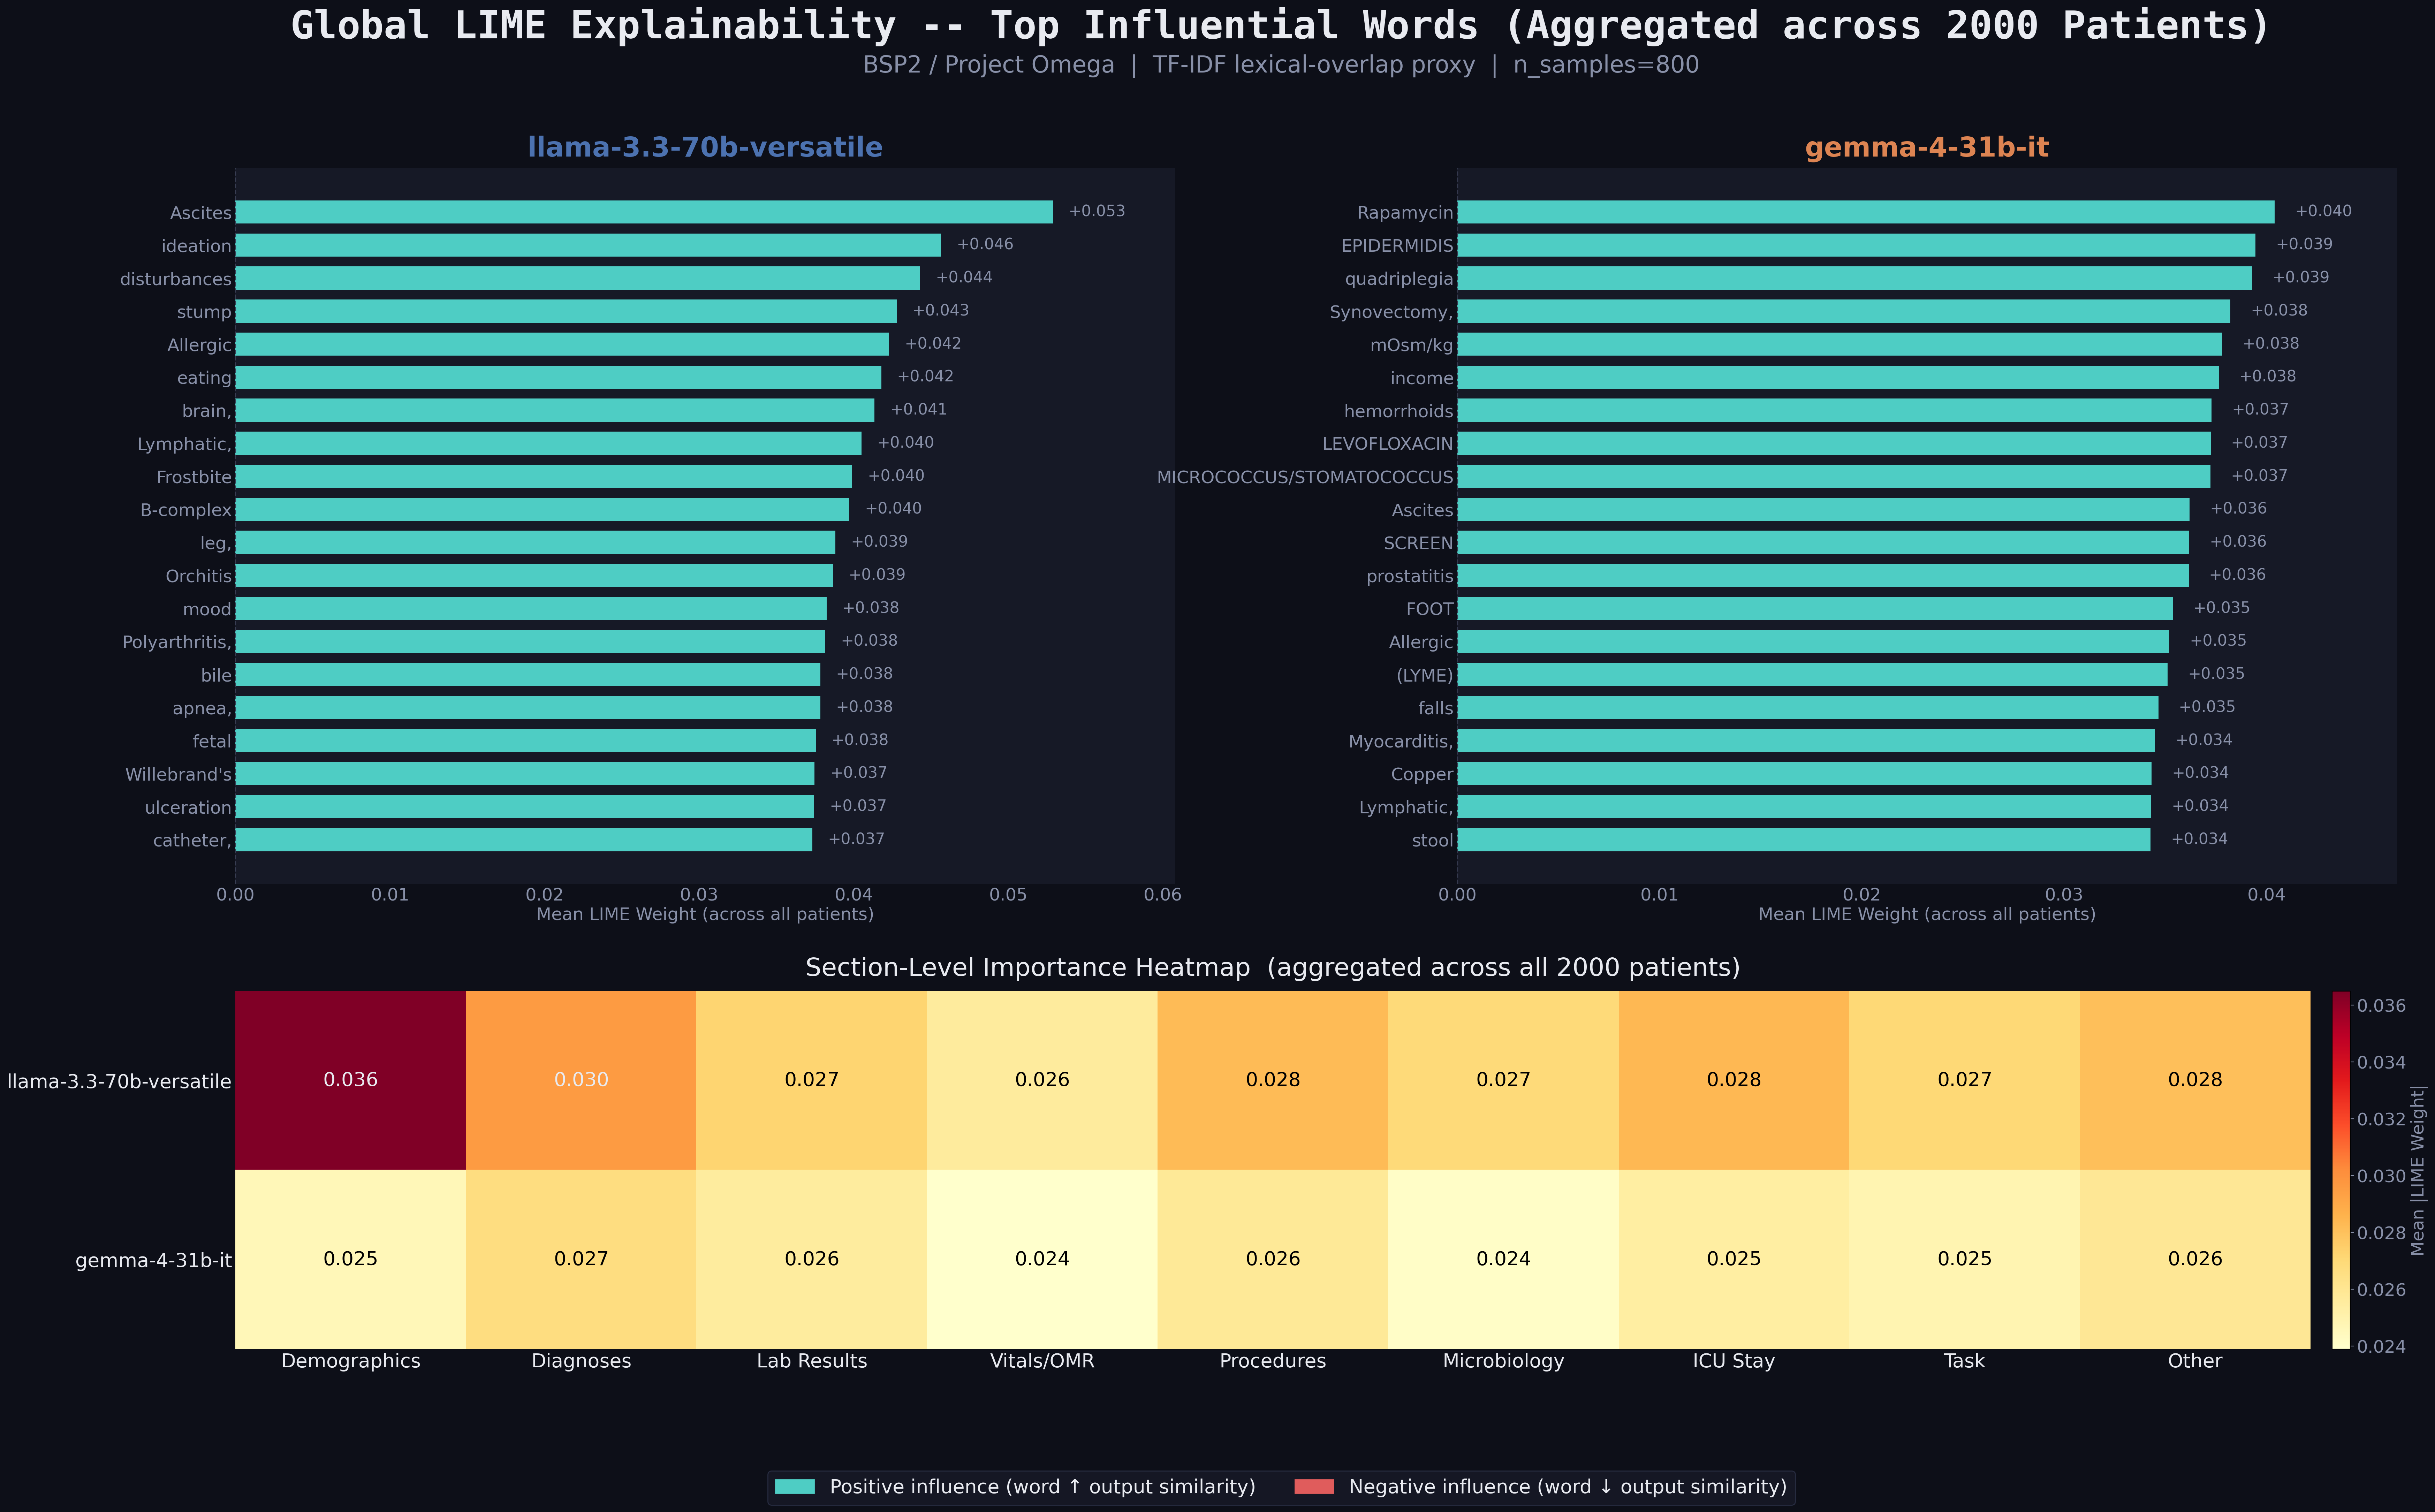
\includegraphics[width=\textwidth]{figures/lime_chart.png}
  \caption{Global LIME explainability results for LLaMA-3.3-70B (left) and Gemma-4-31B (right), aggregated across 50 patients each. Bars show mean absolute influence weight; color indicates direction (teal: positive influence, coral: negative influence). Bottom panels show section-level importance heatmaps.}
  \label{fig:lime}
\end{figure*}

%% =====================================================================
\section{Discussion and Limitations}
%% =====================================================================

\subsection{Discussion}
Three key findings emerge from this study. First, the brevity effect demonstrates that standard automatic metrics can produce misleading model rankings for clinical text generation. Shorter outputs that closely mirror reference diagnosis strings score higher on BLEU and ROUGE, despite being clinically inferior. This result advocates for multi-dimensional LLM-based evaluation as the standard for clinical text generation benchmarks.

Second, Gemma-4-31B's comprehensive output style, characterized by detailed treatment justifications, explicit safety warnings, and structured confidence ratings, is strongly preferred by an autonomous clinical evaluator across all four quality dimensions. The 97.9\% head-to-head win rate across 2,000 patients is a robust result that substantially reduces the influence of prompt-level variance.

Third, the temperature sensitivity experiment demonstrates that Gemma-4-31B produces consistently quality outputs across $T \in \{0.1, 0.5, 1.0\}$, with only marginal variation in lexical diversity metrics. This robustness is practically significant for clinical deployment pipelines operating under fixed inference configurations.

\subsection{Limitations}
The LIME explainability analysis employs a lexical-overlap proxy rather than true semantic attribution. Future work should apply gradient-based attribution methods for more rigorous interpretability.

Drug overlap relies on fuzzy string matching, which may both over-count matches between pharmacologically unrelated drugs sharing similar character sequences, and under-count paraphrased or abbreviated drug names. A standardized pharmacological ontology such as RxNorm would yield more precise recall measurements.

The autonomous evaluator may introduce preference biases, potentially favoring well-structured, verbose outputs independent of actual clinical correctness. Human expert validation by practicing clinicians would substantially strengthen evaluation validity.

Finally, our cohort represents a single institution and a historical time period (2008-2024). Generalizability to contemporary clinical settings and diverse healthcare systems requires validation on more recent and multi-institutional datasets.

%% =====================================================================
\section{Conclusion}
%% =====================================================================

This paper presents Project Omega, a comprehensive evaluation of LLaMA-3.3-70B and Gemma-4-31B for clinical diagnosis hypothesization and treatment recommendation on 2,000 MIMIC-IV patient admissions. Our pipeline combines drug overlap analysis, lexical similarity metrics, LLM-based clinical quality assessment, temperature sensitivity experiments, and LIME explainability analysis into a reproducible evaluation framework.

Gemma-4-31B substantially outperforms LLaMA-3.3-70B in clinical quality, winning 97.9\% of head-to-head evaluations, while simultaneously scoring lower on BLEU and ROUGE. This contradiction resolves when output verbosity is considered: Gemma's longer, more comprehensive outputs are penalized by n-gram metrics that reward lexical conciseness relative to short ICD reference strings. This finding has direct implications for how clinical text generation systems should be evaluated, and motivates the adoption of multi-dimensional LLM-based evaluation frameworks alongside traditional metrics.

Future work should include validation by practicing clinicians, evaluation on contemporary multi-institutional datasets, fine-tuning on clinical corpora, and targeted assessment of safety-critical patient subpopulations such as pediatric or oncological cases.

%% =====================================================================
\begin{thebibliography}{12}

\bibitem{clinicalbert}
Emily Alsentzer, John Murphy, Willie Boag, Wei-Hung Weng, Di Jindi, Tristan Naumann, and Matthew McDermott.
\newblock Publicly available clinical BERT embeddings.
\newblock \emph{arXiv preprint arXiv:1904.03323}, 2019.

\bibitem{gemma}
Gemma Team et al.
\newblock Gemma: Open models based on Gemini research and technology.
\newblock \emph{arXiv preprint arXiv:2403.08295}, 2024.

\bibitem{llama3}
Aaron Grattafiori et al.
\newblock The Llama 3 herd of models.
\newblock \emph{arXiv preprint arXiv:2407.21783}, 2024.

\bibitem{medqa}
Di Jin, Eileen Pan, Nassim Oufattole, Wei-Hung Weng, Hanyi Fang, and Peter Szolovits.
\newblock What disease does this patient have? A large-scale open domain question answering dataset from medical exams.
\newblock \emph{Applied Sciences}, 11(14):6421, 2021.

\bibitem{mimic4}
Alistair Johnson, Lucas Bulgarelli, Tom Pollard, Brian Gow, Benjamin Moody, Steven Horng, Leo Anthony Celi, and Roger Mark.
\newblock MIMIC-IV (version 3.1).
\newblock \emph{PhysioNet}, 2024. doi: 10.13026/kpb9-mt58.

\bibitem{biobert}
Jinhyuk Lee, Wonjin Yoon, Sungdong Kim, Donghyeon Kim, Sunkyu Kim, Chan Ho So, and Jaewoo Kang.
\newblock BioBERT: a pre-trained biomedical language representation model for biomedical text mining.
\newblock \emph{Bioinformatics}, 36(4):1234--1240, 2020.

\bibitem{rouge}
Chin-Yew Lin.
\newblock ROUGE: A package for automatic evaluation of summaries.
\newblock In \emph{Text Summarization Branches Out}, pages 74--81, 2004.

\bibitem{gpt4med}
Harsha Nori, Nicholas King, Scott Mayer McKinney, Dean Carignan, and Eric Horvitz.
\newblock Capabilities of GPT-4 on medical challenge problems.
\newblock \emph{arXiv preprint arXiv:2303.13375}, 2023.

\bibitem{bleu}
Kishore Papineni, Salim Roukos, Todd Ward, and Wei-Jing Zhu.
\newblock BLEU: a method for automatic evaluation of machine translation.
\newblock In \emph{Proceedings of ACL 2002}, pages 311--318, 2002.

\bibitem{lime}
Marco Tulio Ribeiro, Sameer Singh, and Carlos Guestrin.
\newblock ``Why should I trust you?'': Explaining the predictions of any classifier.
\newblock In \emph{Proceedings of ACM KDD 2016}, pages 1135--1144, 2016.

\bibitem{llmclinical}
Karan Singhal, Shekoofeh Azizi, Tao Tu, S.~Sara Mahdavi, Jason Wei, Hyung Won Chung, Nathan Scales, Ajay Tanwani, Heather Cole-Lewis, Stephen Pfohl, et al.
\newblock Large language models encode clinical knowledge.
\newblock \emph{Nature}, 620:172--180, 2023.

\bibitem{llmjudge}
Lianmin Zheng, Wei-Lin Chiang, Ying Sheng, Siyuan Zhuang, Zhanghao Wu, Yonghao Zhuang, Zi Lin, Zhuohan Li, Dacheng Li, Eric P.~Xing, Hao Zhang, Joseph E.~Gonzalez, and Ion Stoica.
\newblock Judging LLM-as-a-Judge with MT-Bench and Chatbot Arena.
\newblock In \emph{Advances in Neural Information Processing Systems}, volume~36, 2023.

\end{thebibliography}

\end{document}
